\section{System design}
(recommended size: 1.5 pages)

\subsection{System overview}
Describe the design of your system, including the system
operation, fault tolerance, and scalability components (which correspond to the
homonym features required by the WantGame CTO).

Describe component of the system, then describe following three scenarios 

\subsubsection*{(Dis)connecting clients}
client connects (scalable?,fault-tolerant) + disconnect is roughly the same

\begin{figure}[h!]
  \centering
    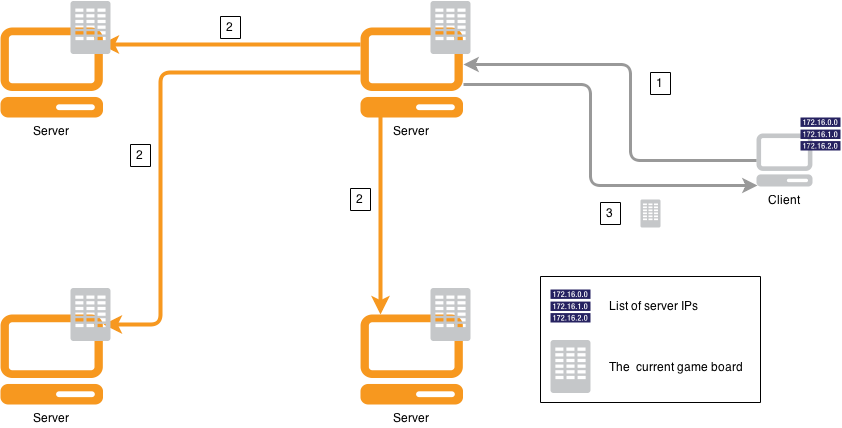
\includegraphics[width=\textwidth]{diagrams/connecting-client}
    
  \caption{A client connecting to a server}
  \label{connect_diagram}
\end{figure}

\subsubsection*{Clients performing actions}
client sends game update (consistency, fault-tolerant when messages are lost)

\begin{figure}[h!]
  \centering
    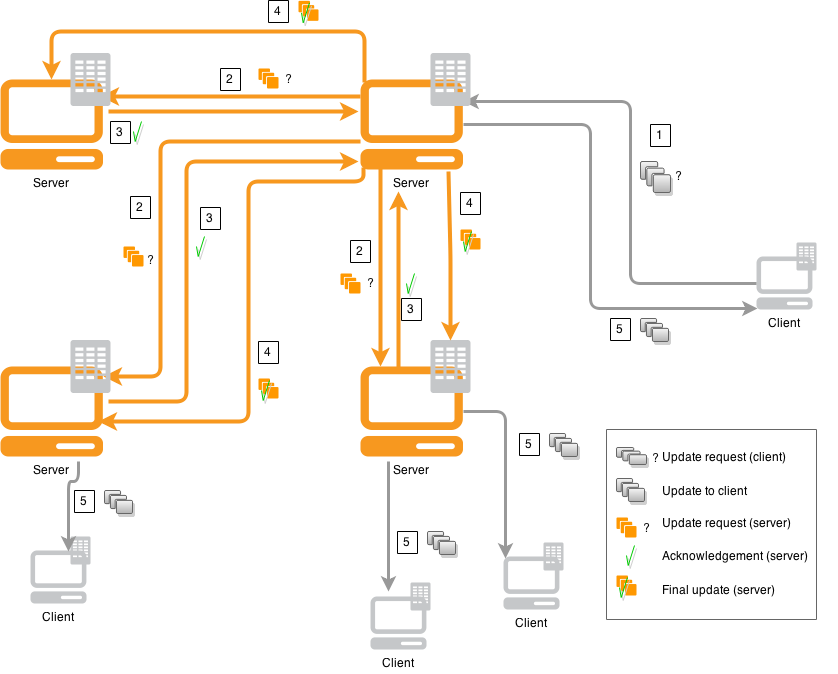
\includegraphics[width=\textwidth]{diagrams/game-update}
    
  \caption{A client sending an update to a server}
  \label{update_diagram}
\end{figure}

\subsubsection*{Client and server crashes}
crashing clients and/or servers (fault-tolerant)

\subsection{Additional System Features}
(optional): Describe each additional feature of your system, one sub-section per feature
 